\chapter{实验}

以下实验使用多种不同分布的数据集,比较多种在 MapReduce 框架下计算数据立方的方法。实验结果表明,没有任何一种方法是``万能”的,根据不同的度量函数、数据分布,不同的方法各有优势。

\section{实验环境}

节点数为7,reducer的数量为20。(此处为完成,之后再补充)

\section{实验数据集与度量}

实验的数据集使用前两个章节提到的具有层次型的数据集,如图 \ref{dataset_table} 所示。表中共有 6 个维属性,分别是 country,state,city,topic,category,subcategory。其中\textless country, state, city\textgreater 是具有层次型的,同理\textless topic, category, subcategory\textgreater 也是具有层次性的。因此在 GroupBy 时,GroupBy(country, state, topic) 和 GroupBy(state, topic)是等价的。并且不会出现 GroupBy(country, city, topic) 这样的跨越层次的操作。该数据集对应的 lattice 如图 \ref{dataset_lattice} 所示。

\begin{figure}[!htb]
\centering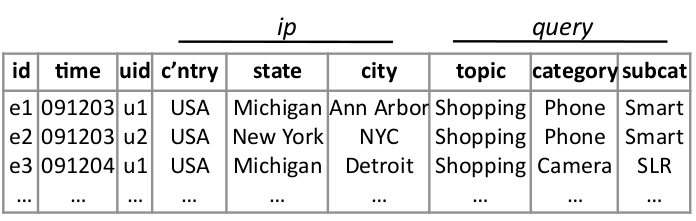
\includegraphics[width=3.5in]{picture/ch_datacube_mr/dataset_table} 
\caption{数据集的表结构}\label{dataset_table} 
\end{figure} 

\begin{figure}[!htb]
\centering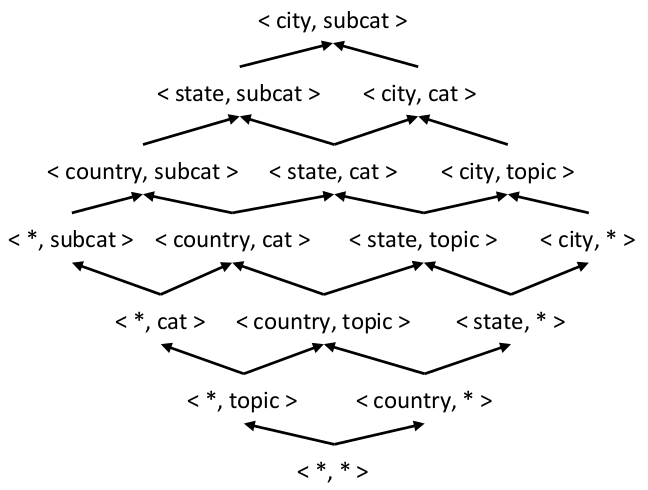
\includegraphics[width=3in]{picture/ch_datacube_mr/dataset_lattice} 
\caption{数据集的lattice}\label{dataset_lattice} 
\end{figure} 

对于这个数据集,实验中使用了3种数据分布。分别如下:
\begin{itemize}

\item \textbf{D1}

对于属性 country 的取值范围为 [1,3],且是均匀分布的。对于属性 topic 的取值范围为[1,10],且是均匀分布的。剩余的属性取值范围较大,如city取值范围为[1,4000],subcategory 取值范围为[1,20000],且都是均匀分布的。由于country和topic的取值范围较小,因此Region(country)和Region(topic)在数据量较大的数据集中均包含了大的group。

\item \textbf{D2A}

为了出现极端的情况,即每个region中都有reducer-unfriendly的group,数据集中的数据是2/8分。即该数据集中有80\%的记录都是相同的,剩下的20\%的数据的分布与\textbf{d1}相同。属性 uid 是均匀分布的。

\item \textbf{D2B}

d2B的数据分布与d2A基本一致,但 uid 是倾斜分布的,也就是会导致求余的划分方式不均匀。

\end{itemize}

这三种数据集都有不同程度的倾斜,D1的倾斜度没有D2的明显,并且D1数据集中仅有部分的region是reducer-unfriendly的,例如Region(country)、Region(topic)。对于以上三种分布,属性 uid 的取值范围均为$[1,{10}^{6}]$。

实验中分别对非整体性度量与整体性度量进行比较,代数度量选择 COUNT(*), 整体性度量选择 COUNT(DISTINCT(uid))。

数据集中记录的数量分别为${10}^{6}$、${10}^{7}$、${10}^{8}$、${10}^{9}$。对于${10}^{9}$的数据集,大小约为45G。


\section{比较算法}

TSP-Cube 除了与 Naive 和 MR-Cube 的方法比较外,还将与 Naive+BatchArea 与 TopDownCube \cite{lee2012efficient} 进行比较。

Naive+BatchArea 是不对数据进行划分,只对 lattice 进行划分,划分的方法与 TSP-Cube 的一致。使用pipesort在一个reduce函数内计算多个group。将TSP-Cube与这个方法对比,是查看当数据倾斜时,数据划分是否能提升计算效率。

TopDownCube,是将 pipesort 与 MapReduce 结合的一种方法。pipsort最根本的思想是对``数据”不断地排序,这个``数据”可能是原数据,也可能是已经计算好GroupBy的数据。TopDownCube沿用了\cite{agarwal1996computation} 中构造pipe树的方法,并且使用 MapReduce 对每个pipeline中的数据按照第一个 region 的属性顺序进行排序。这个方法的缺点是需要执行多次MapReduce,因为对于每个 pipeline都要执行一次 MapReduce。但它可以将多个 region 放在同一个 reducer 上计算,并且由于不是排序都基于原数据,因此产生的中间数据比 Naive+BatchArea要少。这种方法更适合代数度量函数的计算。

对这几种算法的比较的主要包括,在不同的数据分布以及数据大小下,算法的运行时间, 各个reducer输入的记录数。通过算法的运行时间比较各个算法的效率,通过各个 reducer 输入的记录数查看数据划分对各个reducer 之间的负载均衡影响。最后还比较了 TSP-Cube 3次MapReduce各占的比例。

实验代码GtiHub地址:\url{https://github.com/abcdmyz/MapReduceDataCube}

\section{实验结果}

\subsection{DISTINCT 度量}


图\ref{d1_distinct_time}、 \ref{d2a_distinct_time}、 \ref{d2b_distinct_time} 分别为d1, d2A, d2B 三种不同的分布下,5种方法的运行时间比较。图中的横轴为数据大小,图中的纵轴为运行时间,单位为分钟。从图中可看出,当数据量较小时,5种方法之间的差距并不大,当数据量到达${10}^{9}$时,各种方法之间才有较为明显的差距。图\ref{d1_distinct_input}、图\ref{d2a_distinct_input}、图\ref{d2b_distinct_input} 分别为数据大小为${10}^{9}$时,各种方法中各个reducer输入的记录数。从这个记录数查看各个reducer之间的负载差距。

Naive 无论在任何一种分布下所花费的时间都是最多的。D1的数据分布下,Naive+BatchArea的方法的运行时间是最短的。但在D2的分布下,Naive+BatchArea的性能则大打折扣。这是因为对于极端倾斜的数据,就算在Naive的基础上加上了BatchArea,但数据没有进行划分,导致 reducer之间的负载差距过大,仍然会使性能下降。由于D2的倾斜性比D1明显,因此Naive+BatchArea的缺点在D2中更能体现。从图\ref{d2a_distinct_input}和图\ref{d2b_distinct_input} 可看出 Naive+BatchArea 的方法各个reducer输入的数据量有较大的差距,尤其有3个reducer输入的数据量特别大,导致了整体的执行时间变长。

对于 TopDownCube的方法,在D1中仅比Naive的方法好,这是因为它要进行多次的MapReduce对数据进行排序,但uid的取值范围较大,中间数据仅减少了小部分,因此它需要较长的运行时间。而在D2A分布中,它比Naive+BatchArea的方法有优势,这是因为它多次MapReduce产生的中间数据比Naive产生的中间数据要更少,所以相对有一定的优势。但与TPS-Cube相比,在任何一种数据分布中,运行时间都比TSP-Cube的要长,这也是因为数据倾斜导致的。因为TopDown没有对数据进行划分,reducer之间的负载差距依然存在,即使它使用多轮MapReduce减少中间数据。从图\ref{d1_distinct_input}、图\ref{d2a_distinct_input}可看出TopDownCube中各个reducer之间有一定差距,而TPS-Cube的各个reducer之间是非常均匀的。总体而言,将TopDownCube的方法运用在计算整体性度量函数中,优势并不明显。

对于MR-Cube,在D1和D2A分布中,它与TSP-Cube的差别并不明显,运行时间基本上是差不多的。因为这两种方法都对数据进行了划分,并且也是用了Batch Area,将多个gorup放在同一个reducer中计算,减少中间数据。但在D2B分布中,TSP-Cube的优势则较为明显地体现出来。因为D2B中的uid分布是不均匀的,这样MR-Cube中使用求余的方式对数据进行划分,可能导致划分后数据的不均匀。Reducer之间的负载差距则导致MR-Cube性能的下降。在图\ref{d2a_distinct_input}中 MR-Cube 与 TSP-Cube 各个reducer上的数据都是均匀的,也就是数据划分都是较为均匀的。但是图\ref{d2a_distinct_input}中,由于uid的倾斜性,导致MR-Cube各个reducer分布不均匀,但TSP-Cube方法的各个reducer中的数据依然能够均匀分布。

图\ref{d1_distinct_mr123}和图\ref{d2a_distinct_mr123} 分别为TSP-Cube在D1和D2A数据分布,数据集大小为 ${10}^{9}$ 下,三次MapReduce占总体时间的比例。随着数据量增大,MR1和MR3所占的比例都会减少。因此花费一定代价对数据进行划分从而使数据分配均匀对总体性能的提升是有意义的。

TSP-Cube相对于其他方法并不是``完美无缺”或者各方面``遥遥领先”的,它在一些数据分布下,跟大部分的方法在性能上是差别不大的,但在一些较为极端的数据分布下,它能表现出它的优势。它能对数据进行均匀的划分,令各个reducer伤的数据负载均衡,从而提升计算性能。对数据均匀划分,这也是 TeraSort 思想极为重要的贡献。同时 TSP-Cube 适合在整体性度量函数计算中使用,因为这一类函数对于数据是无法随意划分和随意压缩计算的,不可避免的会产生大量的中间数据,只有数据达到一定量级,均匀划分才能发挥它的作用。

\begin{figure}[!ht]
\begin{tabular}{cc}

\begin{minipage}[t]{0.5\textwidth}
\centering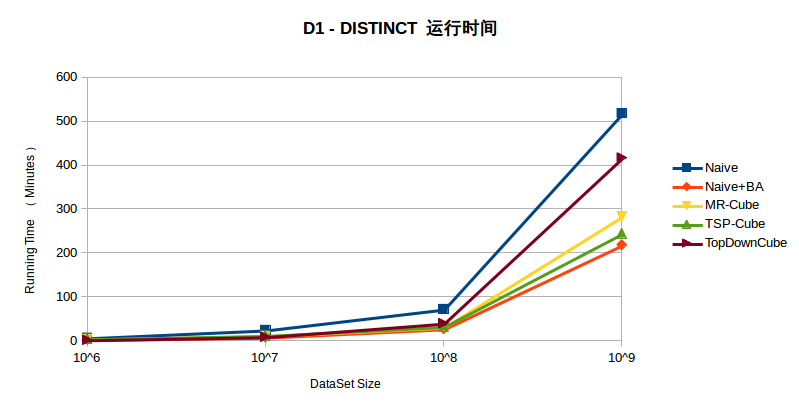
\includegraphics[width=3in]{picture/ch_experiment/d1_distinct_time} 
\caption{D1-DISTINCT 运行时间}\label{d1_distinct_time} 
\end{minipage}

\begin{minipage}[t]{0.5\textwidth}
\centering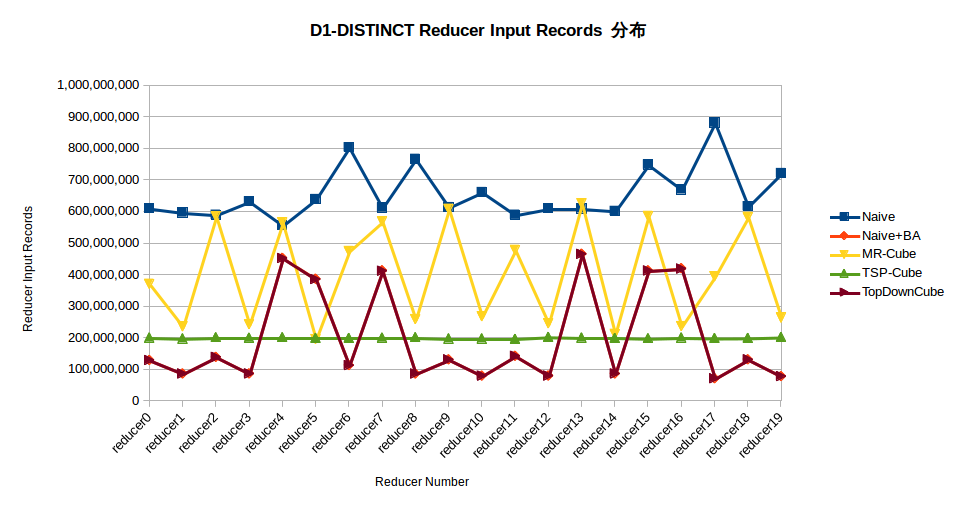
\includegraphics[width=3in]{picture/ch_experiment/d1_distinct_input} 
\caption{D1-DISTINCT Reducer Input}\label{d1_distinct_input} 
\end{minipage}

\end{tabular}
\end{figure}



\begin{figure}[!ht]
\begin{tabular}{cc}

\begin{minipage}[t]{0.5\textwidth}
\centering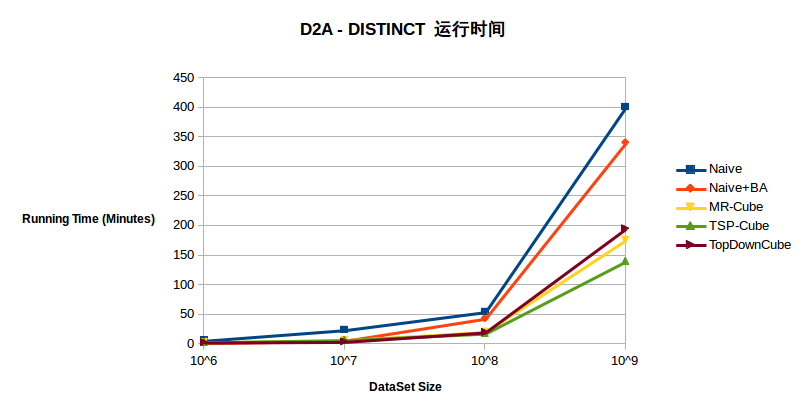
\includegraphics[width=3in]{picture/ch_experiment/d2a_distinct_time} 
\caption{D2A-DISTINCT 运行时间}\label{d2a_distinct_time} 
\end{minipage}

\begin{minipage}[t]{0.5\textwidth}
\centering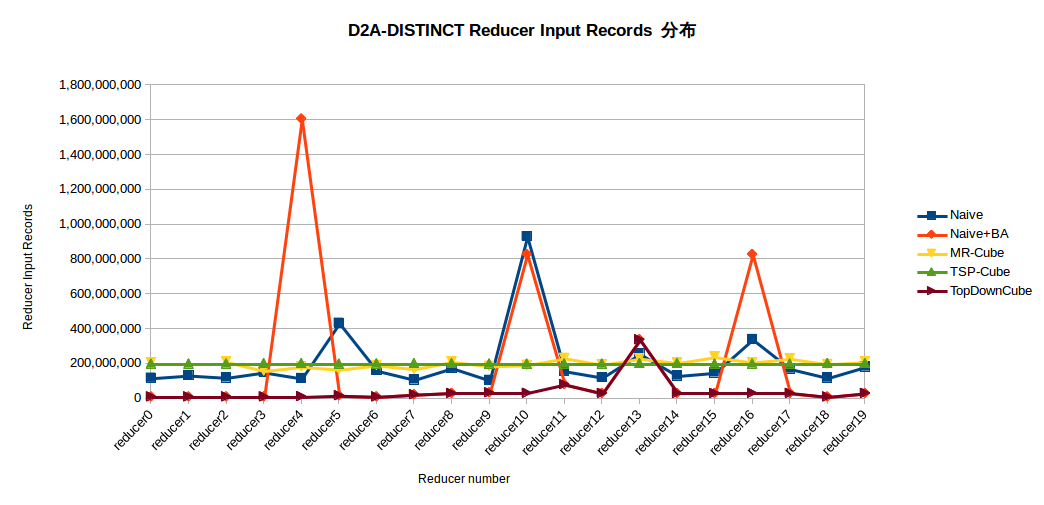
\includegraphics[width=3in]{picture/ch_experiment/d2a_distinct_input} 
\caption{D2A-DISTINCT Reducer Input}\label{d2a_distinct_input} 
\end{minipage}

\end{tabular}
\end{figure}


\begin{figure}[!ht]
\begin{tabular}{cc}

\begin{minipage}[t]{0.5\textwidth}
\centering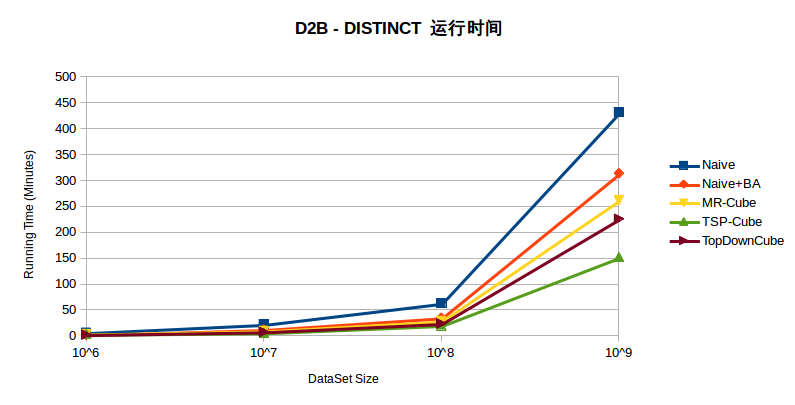
\includegraphics[width=3in]{picture/ch_experiment/d2b_distinct_time} 
\caption{D2B-DISTINCT 运行时间}\label{d2b_distinct_time} 
\end{minipage}

\begin{minipage}[t]{0.5\textwidth}
\centering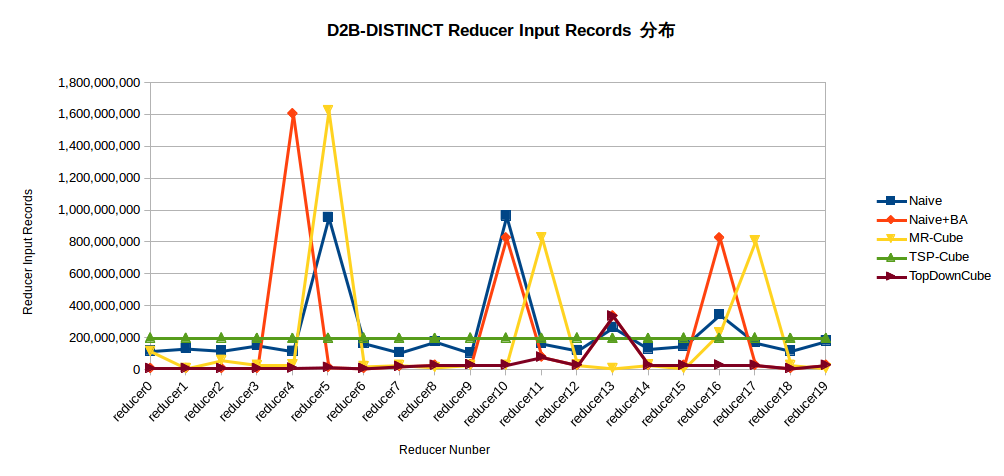
\includegraphics[width=3in]{picture/ch_experiment/d2b_distinct_input} 
\caption{D2B-DISTINCT Reducer Input}\label{d2b_distinct_input} 
\end{minipage}

\end{tabular}
\end{figure}


\begin{figure}[!ht]
\begin{tabular}{cc}

\begin{minipage}[t]{0.5\textwidth}
\centering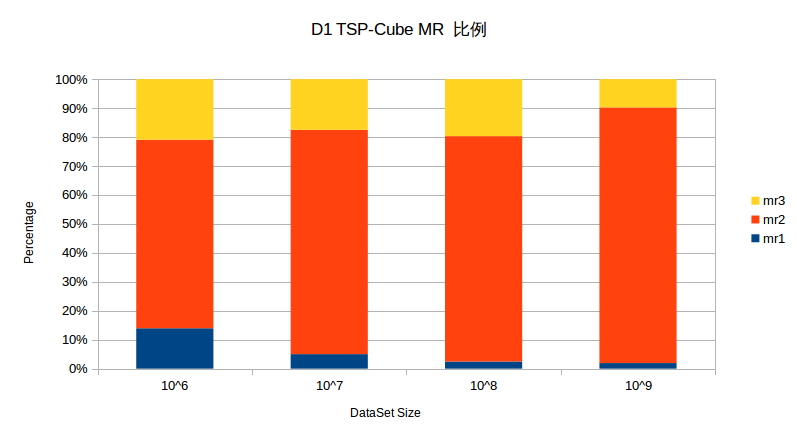
\includegraphics[width=3in]{picture/ch_experiment/d1_distinct_mr123} 
\caption{D1-DISTINCT TSP-CUBE MR 比例}\label{d1_distinct_mr123} 
\end{minipage}

\begin{minipage}[t]{0.5\textwidth}
\centering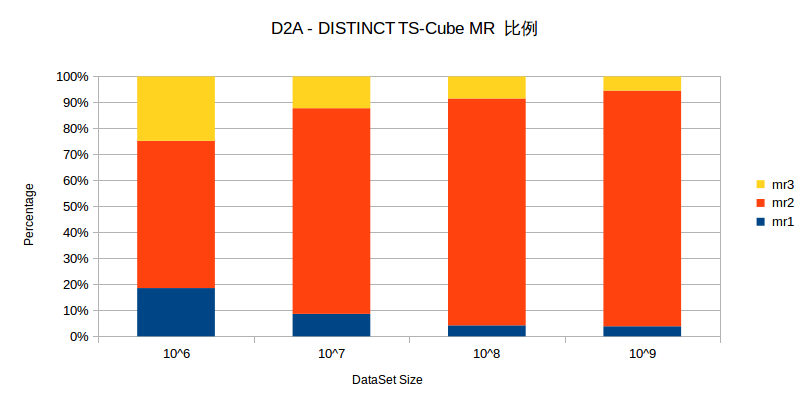
\includegraphics[width=3in]{picture/ch_experiment/d2a_distinct_mr123} 
\caption{D2A-DISTINCT TSP-CUBE MR 比例}\label{d2a_distinct_mr123} 
\end{minipage}

\end{tabular}
\end{figure}



\subsection{COUNT 度量}

在实验中加入代数度量进行对比,是想要说明没有任何一种方法是万能的,就算TSP-Cube能对数据进行均匀划分,也是需要场景的。因此不同的场景下不同的度量函数,应该使用不同的计算方法。以下将5种方法计算COUNT的性能进行比较。图\ref{d1_count_time}、图\ref{d2a_count_time}分别为d1和d2A分布下,5种方法在不同数据大小下的运行时间。图\ref{d1_count_input}、图\ref{d2a_count_input}为不d1和d2A分部下,5种方法各个reducer输入的数据量。

从这些图中发现,在DISTINCT度量中表现最差的Naive,在COUNT度量中却是性能最好的。图\ref{d1_count_time} 中,Naive的点与TopDownCube是重合的。在DISTINCT度量中,Naive方法在reducer上的数据是分布非常不均匀的,但是在COUNT度量中,Naive方法在reducer上的数据分布却是非常均匀的。而TSP-Cube和MR-Cube对数据的划分反而导致数据的不均匀。

这个结果的出现与度量函数本身,还有MapReduce框架的特性有非常大的关系。COUNT是代数度量函数,因此数据可以随意划分,并且对于每个分块进行计算的中间结果都是一个整数,或者数据量是固定的。而MapReduce框架有一个非常重要的特性,Combiner。这个Combiner的作用在上一章节也提到,它等同于本地的reducer。mapper产生的输出并不是直接发给相应的reducer,而是现在本地进行一次reduce计算,再通过网络传输发到reducer上。对于代数函数,一个group内的大量数据都可以变成一条数据发到reducer上,因此中间数据大大减少,并且mapper的数量是有限的,那么分发到一个reducer上一个group内的数据也是有限的。这样有限的数据必然不会导致各个reducer上数据的不均匀。

MR-Cube与TSP-Cube的提出,都是为了解决reducer上数据分配不均匀,差别过大的问题,但在代数度量中,这个问题不存在,那么强行使用这两种方法只会带来更差的性能。从图中也可看出,Naive和TopDownCube在性能上比MR-Cube和TSP-Cube更有优势。

Naive+BatchArea的方法反而还比不上Naive的方法,即使Naive+BatchArea的方法中间数据变少了,但性能反而比Naive的差。这是因为BatchArea需要对数据进行排序,才可执行pipesort的计算。MapReduce默认会对key进行排序,但是对于value,若用户不重载相关函数,value是不会排序的。而pipesort是需要对value进行排序,这里需要花费一定的时间。因此即使Naive的中间数据比Naive+BatchArea多,但因为Naive不需要对value进行排序,因此在性能上能比Naive+BatchArea的有优势。

\begin{figure}[!ht]
\begin{tabular}{cc}

\begin{minipage}[t]{0.5\textwidth}
\centering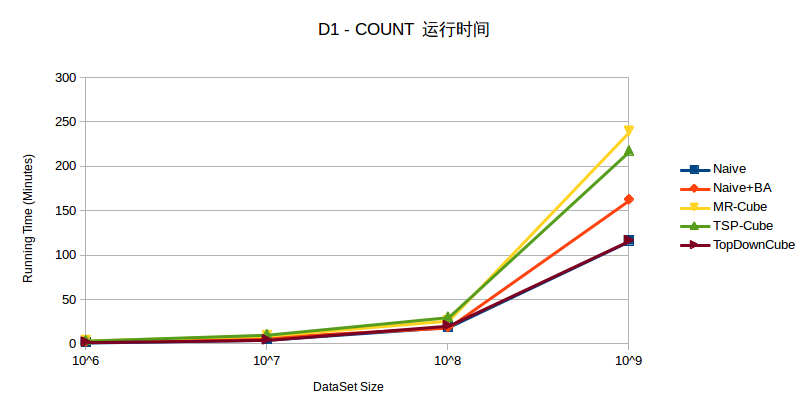
\includegraphics[width=3in]{picture/ch_experiment/d1_count_time} 
\caption{D1-COUNT 运行时间}\label{d1_count_time} 
\end{minipage}

\begin{minipage}[t]{0.5\textwidth}
\centering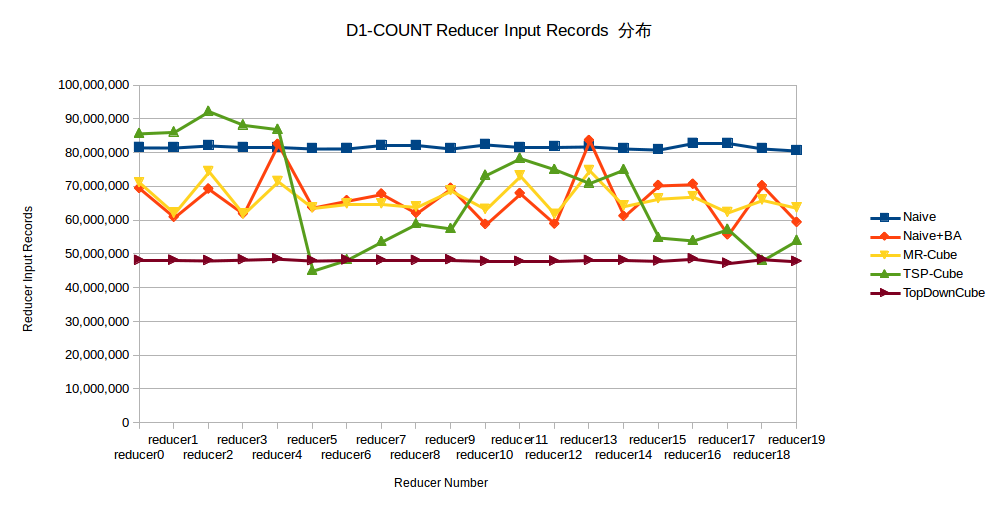
\includegraphics[width=3in]{picture/ch_experiment/d1_count_input} 
\caption{D1-COUNT Reducer Input}\label{d1_count_input} 
\end{minipage}

\end{tabular}
\end{figure}


\begin{figure}[!ht]
\begin{tabular}{cc}

\begin{minipage}[t]{0.5\textwidth}
\centering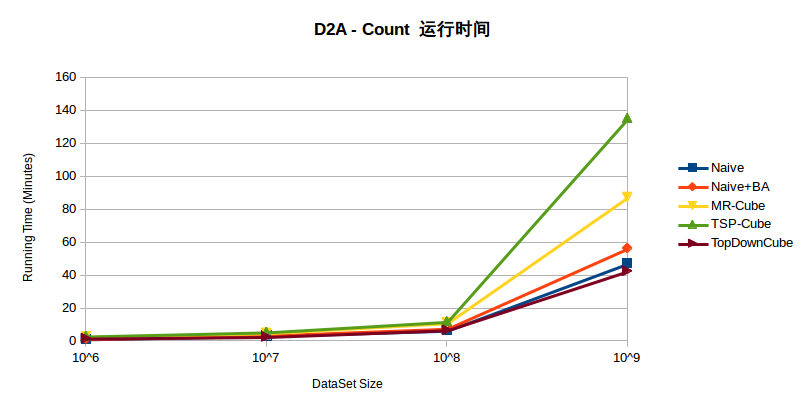
\includegraphics[width=3in]{picture/ch_experiment/d2a_count_time} 
\caption{D2A-COUNT 运行时间}\label{d2a_count_time} 
\end{minipage}

\begin{minipage}[t]{0.5\textwidth}
\centering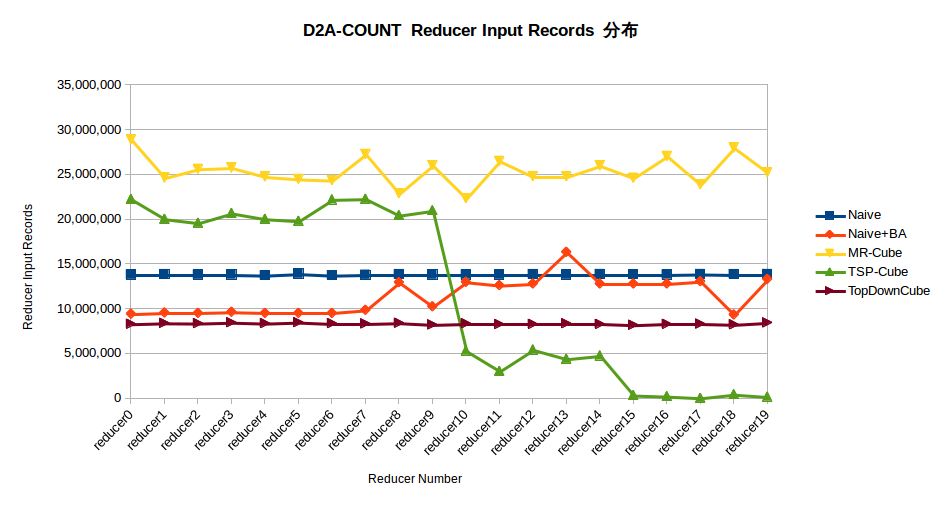
\includegraphics[width=3in]{picture/ch_experiment/d2a_count_input} 
\caption{D2A-COUNT Reducer Input}\label{d2a_count_input} 
\end{minipage}

\end{tabular}
\end{figure}

\section{实验结论}

根据以上的实验,首先得出的一个结论是,TSP-Cube并不是万能的。其次,不同的度量函数使用不同的方法会有不同的结果,目前没有一种方法能对于所有的数据分布、所有的度量都适用。在对一种方法进行评估时,需要考虑到它使用的场景,还需要结合它所基于的框架的特性,来综合评估这种方法。Naive的方法即使简单,也并不是一无是处,结合框架的特性反而能让它发挥优势。而相对复杂的TSP-Cube方法,则着重于解决一些Naive解决不了的更为极端的情况。

对于代数度量,使用Naive的方法已经足够了。Naive方法实现简单,并且在代数度量中,并不会出现reducer负载不均衡的情况。而对于代数度量,虽然TSP-Cube与其他方法相比,没有``遥遥领先”的优势,甚至它在一些场景下与MR-Cube,Naive+BatchArea的性能是差不多的,但是它比这两种方法相比,能处理更多极端的场景,因此建议对于代数度量函数,可使用TSP-Cube的方法。


